\PassOptionsToPackage{unicode=true}{hyperref} % options for packages loaded elsewhere
\PassOptionsToPackage{hyphens}{url}
%
\documentclass[]{ctexart}
\usepackage{lmodern}
\usepackage{amssymb,amsmath}
\usepackage{ifxetex,ifluatex}
\usepackage{fixltx2e} % provides \textsubscript
\ifnum 0\ifxetex 1\fi\ifluatex 1\fi=0 % if pdftex
  \usepackage[T1]{fontenc}
  \usepackage[utf8]{inputenc}
  \usepackage{textcomp} % provides euro and other symbols
\else % if luatex or xelatex
  \usepackage{unicode-math}
  \defaultfontfeatures{Ligatures=TeX,Scale=MatchLowercase}
    \setmonofont[Mapping=tex-ansi]{Fira Mono}
\fi
% use upquote if available, for straight quotes in verbatim environments
\IfFileExists{upquote.sty}{\usepackage{upquote}}{}
% use microtype if available
\IfFileExists{microtype.sty}{%
\usepackage[]{microtype}
\UseMicrotypeSet[protrusion]{basicmath} % disable protrusion for tt fonts
}{}
\IfFileExists{parskip.sty}{%
\usepackage{parskip}
}{% else
\setlength{\parindent}{0pt}
\setlength{\parskip}{6pt plus 2pt minus 1pt}
}
\usepackage{hyperref}
\hypersetup{
            pdftitle={一带一路对中国和其他沿线国家的影响及政策分析},
            pdfauthor={范皓年; 邓睿哲; 李润泽},
            pdfborder={0 0 0},
            breaklinks=true}
\urlstyle{same}  % don't use monospace font for urls
\usepackage[left=2cm, right=2cm, top=2.5cm, bottom=2.5cm]{geometry}
\usepackage{color}
\usepackage{fancyvrb}
\newcommand{\VerbBar}{|}
\newcommand{\VERB}{\Verb[commandchars=\\\{\}]}
\DefineVerbatimEnvironment{Highlighting}{Verbatim}{commandchars=\\\{\}}
% Add ',fontsize=\small' for more characters per line
\usepackage{framed}
\definecolor{shadecolor}{RGB}{248,248,248}
\newenvironment{Shaded}{\begin{snugshade}}{\end{snugshade}}
\newcommand{\AlertTok}[1]{\textcolor[rgb]{0.94,0.16,0.16}{#1}}
\newcommand{\AnnotationTok}[1]{\textcolor[rgb]{0.56,0.35,0.01}{\textbf{\textit{#1}}}}
\newcommand{\AttributeTok}[1]{\textcolor[rgb]{0.77,0.63,0.00}{#1}}
\newcommand{\BaseNTok}[1]{\textcolor[rgb]{0.00,0.00,0.81}{#1}}
\newcommand{\BuiltInTok}[1]{#1}
\newcommand{\CharTok}[1]{\textcolor[rgb]{0.31,0.60,0.02}{#1}}
\newcommand{\CommentTok}[1]{\textcolor[rgb]{0.56,0.35,0.01}{\textit{#1}}}
\newcommand{\CommentVarTok}[1]{\textcolor[rgb]{0.56,0.35,0.01}{\textbf{\textit{#1}}}}
\newcommand{\ConstantTok}[1]{\textcolor[rgb]{0.00,0.00,0.00}{#1}}
\newcommand{\ControlFlowTok}[1]{\textcolor[rgb]{0.13,0.29,0.53}{\textbf{#1}}}
\newcommand{\DataTypeTok}[1]{\textcolor[rgb]{0.13,0.29,0.53}{#1}}
\newcommand{\DecValTok}[1]{\textcolor[rgb]{0.00,0.00,0.81}{#1}}
\newcommand{\DocumentationTok}[1]{\textcolor[rgb]{0.56,0.35,0.01}{\textbf{\textit{#1}}}}
\newcommand{\ErrorTok}[1]{\textcolor[rgb]{0.64,0.00,0.00}{\textbf{#1}}}
\newcommand{\ExtensionTok}[1]{#1}
\newcommand{\FloatTok}[1]{\textcolor[rgb]{0.00,0.00,0.81}{#1}}
\newcommand{\FunctionTok}[1]{\textcolor[rgb]{0.00,0.00,0.00}{#1}}
\newcommand{\ImportTok}[1]{#1}
\newcommand{\InformationTok}[1]{\textcolor[rgb]{0.56,0.35,0.01}{\textbf{\textit{#1}}}}
\newcommand{\KeywordTok}[1]{\textcolor[rgb]{0.13,0.29,0.53}{\textbf{#1}}}
\newcommand{\NormalTok}[1]{#1}
\newcommand{\OperatorTok}[1]{\textcolor[rgb]{0.81,0.36,0.00}{\textbf{#1}}}
\newcommand{\OtherTok}[1]{\textcolor[rgb]{0.56,0.35,0.01}{#1}}
\newcommand{\PreprocessorTok}[1]{\textcolor[rgb]{0.56,0.35,0.01}{\textit{#1}}}
\newcommand{\RegionMarkerTok}[1]{#1}
\newcommand{\SpecialCharTok}[1]{\textcolor[rgb]{0.00,0.00,0.00}{#1}}
\newcommand{\SpecialStringTok}[1]{\textcolor[rgb]{0.31,0.60,0.02}{#1}}
\newcommand{\StringTok}[1]{\textcolor[rgb]{0.31,0.60,0.02}{#1}}
\newcommand{\VariableTok}[1]{\textcolor[rgb]{0.00,0.00,0.00}{#1}}
\newcommand{\VerbatimStringTok}[1]{\textcolor[rgb]{0.31,0.60,0.02}{#1}}
\newcommand{\WarningTok}[1]{\textcolor[rgb]{0.56,0.35,0.01}{\textbf{\textit{#1}}}}
\usepackage{graphicx,grffile}
\makeatletter
\def\maxwidth{\ifdim\Gin@nat@width>\linewidth\linewidth\else\Gin@nat@width\fi}
\def\maxheight{\ifdim\Gin@nat@height>\textheight\textheight\else\Gin@nat@height\fi}
\makeatother
% Scale images if necessary, so that they will not overflow the page
% margins by default, and it is still possible to overwrite the defaults
% using explicit options in \includegraphics[width, height, ...]{}
\setkeys{Gin}{width=\maxwidth,height=\maxheight,keepaspectratio}
\setlength{\emergencystretch}{3em}  % prevent overfull lines
\providecommand{\tightlist}{%
  \setlength{\itemsep}{0pt}\setlength{\parskip}{0pt}}
\setcounter{secnumdepth}{5}
% Redefines (sub)paragraphs to behave more like sections
\ifx\paragraph\undefined\else
\let\oldparagraph\paragraph
\renewcommand{\paragraph}[1]{\oldparagraph{#1}\mbox{}}
\fi
\ifx\subparagraph\undefined\else
\let\oldsubparagraph\subparagraph
\renewcommand{\subparagraph}[1]{\oldsubparagraph{#1}\mbox{}}
\fi

% set default figure placement to htbp
\makeatletter
\def\fps@figure{htbp}
\makeatother

\let\oldhref\href
\renewcommand{\href}[2]{\oldhref{#1}{\textcolor{blue}{\underline{#2}}}}

\let\oldhyperlink\hyperlink
\renewcommand{\hyperlink}[2]{\oldhyperlink{#1}{\textcolor{red}{\underline{#2}}}}
\usepackage{etoolbox}
\makeatletter
\providecommand{\subtitle}[1]{% add subtitle to \maketitle
  \apptocmd{\@title}{\par {\large #1 \par}}{}{}
}
\makeatother

\title{一带一路对中国和其他沿线国家的影响及政策分析}
\providecommand{\subtitle}[1]{}
\subtitle{数据科学的视角}
\author{范皓年 \and 邓睿哲 \and 李润泽\footnote{名拼音序.}}
\date{}

\begin{document}
\maketitle

{
\setcounter{tocdepth}{2}
\tableofcontents
}
\hypertarget{ux524dux8a00}{%
\section{前言}\label{ux524dux8a00}}

\hypertarget{ux6982ux8981}{%
\subsection{概要}\label{ux6982ux8981}}

\hypertarget{ux73afux5883}{%
\subsection{环境}\label{ux73afux5883}}

\hypertarget{r-info}{%
\subsubsection{R info}\label{r-info}}

\begin{verbatim}
## R version 4.1.0 (2021-05-18)
## Platform: x86_64-pc-linux-gnu (64-bit)
## Running under: Ubuntu 20.04.2 LTS
## 
## Locale:
##   LC_CTYPE=zh_CN.UTF-8       LC_NUMERIC=C              
##   LC_TIME=zh_CN.UTF-8        LC_COLLATE=zh_CN.UTF-8    
##   LC_MONETARY=zh_CN.UTF-8    LC_MESSAGES=zh_CN.UTF-8   
##   LC_PAPER=zh_CN.UTF-8       LC_NAME=C                 
##   LC_ADDRESS=C               LC_TELEPHONE=C            
##   LC_MEASUREMENT=zh_CN.UTF-8 LC_IDENTIFICATION=C       
## 
## Package version:
##   dplyr_1.0.6      ggdag_0.2.3      ggplot2_3.3.3    lubridate_1.7.10
##   mice_3.13.0      purrr_0.3.4      readr_1.4.0      showtext_0.9-2  
##   stringr_1.4.0    tidyr_1.1.3      tidyverse_1.3.1  VIM_6.1.0
\end{verbatim}

\hypertarget{python-info}{%
\subsubsection{python info}\label{python-info}}

// TODO

\hypertarget{ux4e3bux8981ux7ed3ux679c}{%
\section{主要结果}\label{ux4e3bux8981ux7ed3ux679c}}

\hypertarget{ux6570ux636eux6a21ux578b}{%
\subsection{数据模型}\label{ux6570ux636eux6a21ux578b}}

我们的数据模型如图所示:

\begin{figure}

{\centering 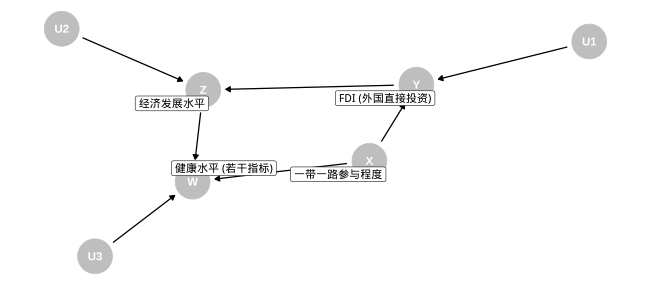
\includegraphics[width=0.65\linewidth,height=0.6\textheight]{resources/DAG} 

}

\caption{数据模型示意图}\label{fig:unnamed-chunk-3}
\end{figure}

此图\textsuperscript{{[}1{]}}是有向无环图(Directed acyclic graph,
DAG),边代表因果作用\textsuperscript{{[}2{]}}.

\begin{figure}

{\centering \includegraphics[width=0.65\linewidth,height=0.6\textheight]{resources/Missing data} 

}

\caption{缺失数据示意图}\label{fig:unnamed-chunk-4}
\end{figure}

\hypertarget{ux5206ux6790}{%
\subsection{分析}\label{ux5206ux6790}}

我们利用(Chernozhukov et al.,
2021)\textsuperscript{{[}3{]}}的方法进行分析.

首先注意到数据集中存在许多缺失数据\textsuperscript{{[}4{]}},使用linear
regression with bootstrap进行缺失数据填补.\textsuperscript{{[}5{]}}

\hypertarget{ux7a0bux5e8f}{%
\subsection{程序}\label{ux7a0bux5e8f}}

\hypertarget{non-standard-evaluation-in-r}{%
\subsubsection{Non-standard evaluation in
R}\label{non-standard-evaluation-in-r}}

\hypertarget{ux5177ux4f53ux6d41ux7a0b}{%
\section{具体流程}\label{ux5177ux4f53ux6d41ux7a0b}}

\hypertarget{the-workflow}{%
\subsection{The Workflow}\label{the-workflow}}

\begin{figure}
\centering
\includegraphics{resources/workflow.png}
\caption[The Data Science Workflow]{The Data Science
Workflow\footnotemark{}}
\end{figure}
\footnotetext{This picture is from \emph{R for Data
  Science}\textsuperscript{{[}6{]}}, released under
  \href{http://creativecommons.org/licenses/by-nc-nd/3.0/us/}{CC
  BY-NC-ND 3.0 US}.}

\hypertarget{import}{%
\subsection{Import}\label{import}}

// 需要数据集的完整描述和获取方式

// TODO - \textbf{R. Li}

\hypertarget{tidy}{%
\subsection{Tidy}\label{tidy}}

tidy data\textsuperscript{{[}7{]}}

\begin{Shaded}
\begin{Highlighting}[]
\NormalTok{raw_df <-}\StringTok{ }\KeywordTok{read_csv}\NormalTok{(}\StringTok{"./data/investment/FDI_untidy.csv"}\NormalTok{)}

\NormalTok{process <-}\StringTok{ }\ControlFlowTok{function}\NormalTok{(raw_df) \{}
\NormalTok{  simplified_df <-}\StringTok{ }\NormalTok{raw_df }\OperatorTok
\StringTok{    }\KeywordTok{filter}\NormalTok{(X1 }\OperatorTok\StringTok{ }\KeywordTok{str_detect}\NormalTok{(}\StringTok{"^}\CharTok{\textbackslash{}\textbackslash{}}\StringTok{d"}\NormalTok{)) }\OperatorTok
\StringTok{    }\KeywordTok{rename}\NormalTok{(时间 =}\StringTok{ }\NormalTok{X1)}

\NormalTok{  fliped_df <-}\StringTok{ }\NormalTok{simplified_df }\OperatorTok
\StringTok{    }\KeywordTok{pivot_longer}\NormalTok{(}\KeywordTok{c}\NormalTok{(}\OperatorTok{-}\NormalTok{时间), }\DataTypeTok{names_to =} \StringTok{"observation"}\NormalTok{, }\DataTypeTok{values_to =} \StringTok{"val"}\NormalTok{)}

\NormalTok{  stdize <-}\StringTok{ }\ControlFlowTok{function}\NormalTok{(str) \{}
\NormalTok{    str }\OperatorTok
\StringTok{      }\KeywordTok{str_replace}\NormalTok{(}\DataTypeTok{pattern =} \StringTok{"(.*):(总计|一带一路)"}\NormalTok{, }\DataTypeTok{replacement =} \StringTok{"}\CharTok{\textbackslash{}\textbackslash{}}\StringTok{1/}\CharTok{\textbackslash{}\textbackslash{}}\StringTok{2/}\CharTok{\textbackslash{}\textbackslash{}}\StringTok{2"}\NormalTok{) }\OperatorTok
\StringTok{      }\KeywordTok{str_replace}\NormalTok{(}\DataTypeTok{pattern =} \StringTok{"::"}\NormalTok{, }\DataTypeTok{replacement =} \StringTok{":"}\NormalTok{) }\OperatorTok
\StringTok{      }\KeywordTok{str_replace}\NormalTok{(}\DataTypeTok{pattern =} \StringTok{"(.*):(.*洲):*(.*)"}\NormalTok{, }\DataTypeTok{replacement =} \StringTok{"}\CharTok{\textbackslash{}\textbackslash{}}\StringTok{1/}\CharTok{\textbackslash{}\textbackslash{}}\StringTok{2/}\CharTok{\textbackslash{}\textbackslash{}}\StringTok{3"}\NormalTok{)}
\NormalTok{  \}}

\NormalTok{  sep_df <-}\StringTok{ }\NormalTok{fliped_df }\OperatorTok
\StringTok{    }\KeywordTok{mutate}\NormalTok{(}\DataTypeTok{observation =}\NormalTok{ observation }\OperatorTok\StringTok{ }\KeywordTok{stdize}\NormalTok{()) }\OperatorTok
\StringTok{    }\KeywordTok{separate}\NormalTok{(}\DataTypeTok{col =} \StringTok{"observation"}\NormalTok{, }\DataTypeTok{into =} \KeywordTok{c}\NormalTok{(}\StringTok{"type"}\NormalTok{, }\StringTok{"地区"}\NormalTok{, }\StringTok{"国家"}\NormalTok{), }\DataTypeTok{sep =} \StringTok{"/"}\NormalTok{)}

\NormalTok{  df <-}\StringTok{ }\NormalTok{sep_df }\OperatorTok\StringTok{ }\KeywordTok{spread}\NormalTok{(}\DataTypeTok{key =} \StringTok{"type"}\NormalTok{, }\DataTypeTok{value =} \StringTok{"val"}\NormalTok{)}
\NormalTok{\}}

\NormalTok{raw_df }\OperatorTok
\StringTok{  }\KeywordTok{process}\NormalTok{() }\OperatorTok
\StringTok{  }\KeywordTok{write_csv}\NormalTok{(}\StringTok{"./data/investment/FDI_tidy.csv"}\NormalTok{)}

\NormalTok{cont <-}\StringTok{ }\NormalTok{raw_df }\OperatorTok
\StringTok{  }\KeywordTok{filter}\NormalTok{(X1 }\OperatorTok{==}\StringTok{ "状态"}\NormalTok{) }\OperatorTok
\StringTok{  }\KeywordTok{as_vector}\NormalTok{() }\OperatorTok
\StringTok{  }\NormalTok{.[. }\OperatorTok{==}\StringTok{ "继续"}\NormalTok{] }\OperatorTok
\StringTok{  }\KeywordTok{names}\NormalTok{()}
\NormalTok{raw_df }\OperatorTok
\StringTok{  }\KeywordTok{select}\NormalTok{(X1, }\KeywordTok{all_of}\NormalTok{(cont)) }\OperatorTok
\StringTok{  }\KeywordTok{process}\NormalTok{() }\OperatorTok
\StringTok{  }\KeywordTok{write_csv}\NormalTok{(}\StringTok{"./data/investment/FDI_tidy_cont.csv"}\NormalTok{)}
\end{Highlighting}
\end{Shaded}

\begin{Shaded}
\begin{Highlighting}[]
\NormalTok{raw_df <-}\StringTok{ }\KeywordTok{read_csv}\NormalTok{(}
  \DataTypeTok{file =} \StringTok{"./data/investment/FDI_tidy_cont.csv"}\NormalTok{,}
  \DataTypeTok{col_types =} \KeywordTok{cols}\NormalTok{(}
\NormalTok{    时间 =}\StringTok{ }\KeywordTok{col_date}\NormalTok{(}\DataTypeTok{format =} \StringTok{"%m/%Y"}\NormalTok{)}
\NormalTok{  ),}
  \DataTypeTok{guess_max =} \DecValTok{50000}
\NormalTok{)}

\NormalTok{df0 <-}\StringTok{ }\NormalTok{raw_df }\OperatorTok
\StringTok{  }\KeywordTok{filter}\NormalTok{(}\OperatorTok{!}\KeywordTok{is.na}\NormalTok{(国家))}

\CommentTok{# 对外直接投资:非金融类:累计 为一带一路数据所特有}
\NormalTok{OBOR_col <-}\StringTok{ "对外直接投资:非金融类:累计"}

\NormalTok{df <-}\StringTok{ }\NormalTok{df0 }\OperatorTok
\StringTok{  }\KeywordTok{filter}\NormalTok{(国家 }\OperatorTok{!=}\StringTok{ "一带一路"} \OperatorTok{&}\StringTok{ }\NormalTok{国家 }\OperatorTok{!=}\StringTok{ "总计"}\NormalTok{) }\OperatorTok
\StringTok{  }\KeywordTok{select}\NormalTok{(}\OperatorTok{-}\KeywordTok{all_of}\NormalTok{(OBOR_col))}

\NormalTok{df <-}\StringTok{ }\NormalTok{df }\OperatorTok
\StringTok{  }\KeywordTok{filter}\NormalTok{(}\KeywordTok{month}\NormalTok{(时间) }\OperatorTok{==}\StringTok{ }\DecValTok{12}\NormalTok{) }\OperatorTok
\StringTok{  }\KeywordTok{mutate}\NormalTok{(年份 =}\StringTok{ }\KeywordTok{as.integer}\NormalTok{(}\KeywordTok{year}\NormalTok{(时间)), }\DataTypeTok{.keep =} \StringTok{"unused"}\NormalTok{, }\DataTypeTok{.before =} \DecValTok{1}\NormalTok{) }\OperatorTok
\StringTok{  }\KeywordTok{filter}\NormalTok{(年份 }\OperatorTok{>=}\StringTok{ }\DecValTok{2002}\NormalTok{)}

\NormalTok{df <-}\StringTok{ }\NormalTok{df }\OperatorTok
\StringTok{  }\KeywordTok{select}\NormalTok{(}\KeywordTok{names}\NormalTok{(df) }\OperatorTok\StringTok{ }\KeywordTok{str_subset}\NormalTok{(}\DataTypeTok{pattern =} \StringTok{"投资(和其他)*$"}\NormalTok{, }\DataTypeTok{negate =} \OtherTok{TRUE}\NormalTok{)) }\OperatorTok
\StringTok{  }\KeywordTok{filter}\NormalTok{(}\OperatorTok{!}\KeywordTok{is.na}\NormalTok{(}\StringTok{`}\DataTypeTok{对外直接投资:截至累计}\StringTok{`}\NormalTok{))}

\NormalTok{df }\OperatorTok\StringTok{ }\KeywordTok{write_csv}\NormalTok{(}\DataTypeTok{file =} \StringTok{"./data/investment/FDI_useful.csv"}\NormalTok{)}

\NormalTok{df1 <-}\StringTok{ }\NormalTok{df0 }\OperatorTok
\StringTok{  }\KeywordTok{filter}\NormalTok{(国家 }\OperatorTok{==}\StringTok{ "一带一路"} \OperatorTok{&}\StringTok{ }\OperatorTok{!}\KeywordTok{is.na}\NormalTok{(.[OBOR_col])) }\OperatorTok
\StringTok{  }\KeywordTok{select}\NormalTok{(时间, }\KeywordTok{all_of}\NormalTok{(OBOR_col)) }\OperatorTok
\StringTok{  }\KeywordTok{mutate}\NormalTok{(}
\NormalTok{    年份 =}\StringTok{ }\KeywordTok{as.integer}\NormalTok{(}\KeywordTok{year}\NormalTok{(时间)),}
\NormalTok{    月份 =}\StringTok{ }\KeywordTok{as.integer}\NormalTok{(}\KeywordTok{month}\NormalTok{(时间)),}
    \DataTypeTok{.keep =} \StringTok{"unused"}\NormalTok{, }\DataTypeTok{.before =} \DecValTok{1}\NormalTok{) }\OperatorTok
\StringTok{  }\KeywordTok{arrange}\NormalTok{(年份, 月份)}

\NormalTok{df1 }\OperatorTok\StringTok{ }\KeywordTok{write_csv}\NormalTok{(}\DataTypeTok{file =} \StringTok{"./data/investment/FDI_OBOR.csv"}\NormalTok{)}
\end{Highlighting}
\end{Shaded}

\hypertarget{understand}{%
\subsection{Understand}\label{understand}}

\begin{Shaded}
\begin{Highlighting}[]
\NormalTok{fdi <-}\StringTok{ }\KeywordTok{read_csv}\NormalTok{(}
  \DataTypeTok{file =} \StringTok{"./data/investment/FDI_useful.csv"}\NormalTok{,}
  \DataTypeTok{col_types =} \KeywordTok{cols}\NormalTok{(}
\NormalTok{    年份 =}\StringTok{ }\KeywordTok{col_double}\NormalTok{(),}
\NormalTok{    国家 =}\StringTok{ }\KeywordTok{col_factor}\NormalTok{()}
\NormalTok{  )}
\NormalTok{) }\OperatorTok\StringTok{ }\KeywordTok{unite}\NormalTok{(}\DataTypeTok{col =}\NormalTok{ 国家, 地区, 国家)}

\NormalTok{country_name <-}\StringTok{ }\NormalTok{fdi[[}\StringTok{"国家"}\NormalTok{]] }\OperatorTok\StringTok{ }\KeywordTok{unique}\NormalTok{()}

\NormalTok{fdi_na <-}\StringTok{ }\NormalTok{fdi }\OperatorTok
\StringTok{  }\NormalTok{tidyr}\OperatorTok{::}\KeywordTok{complete}\NormalTok{(年份, 国家) }\OperatorTok
\StringTok{  }\KeywordTok{rename}\NormalTok{(对外直接投资 =}\StringTok{ `}\DataTypeTok{对外直接投资:截至累计}\StringTok{`}\NormalTok{)}

\NormalTok{fdi_lg <-}\StringTok{ }\NormalTok{fdi_na }\OperatorTok
\StringTok{  }\KeywordTok{mutate}\NormalTok{(}\DataTypeTok{lg =} \KeywordTok{log}\NormalTok{(对外直接投资), }\DataTypeTok{.keep =} \StringTok{"unused"}\NormalTok{)}

\NormalTok{fill_a_country <-}\StringTok{ }\ControlFlowTok{function}\NormalTok{(.dt, .cn) \{}
\NormalTok{  res <-}\StringTok{ }\NormalTok{.dt }\OperatorTok
\StringTok{    }\KeywordTok{filter}\NormalTok{(国家 }\OperatorTok{==}\StringTok{ }\NormalTok{.cn) }\OperatorTok
\StringTok{    }\KeywordTok{mice}\NormalTok{(}\DataTypeTok{method =} \StringTok{"norm.boot"}\NormalTok{, }\DataTypeTok{m =} \DecValTok{1}\NormalTok{, }\DataTypeTok{maxit =} \DecValTok{3}\NormalTok{) }\OperatorTok
\StringTok{    }\KeywordTok{complete}\NormalTok{()}
  \ControlFlowTok{if}\NormalTok{ (}\KeywordTok{any}\NormalTok{(}\KeywordTok{is.na}\NormalTok{(res}\OperatorTok{$}\NormalTok{lg))) \{}
\NormalTok{    non_na <-}\StringTok{ }\OperatorTok{!}\NormalTok{(res}\OperatorTok{$}\NormalTok{lg }\OperatorTok\StringTok{ }\KeywordTok{is.na}\NormalTok{())}
\NormalTok{    res}\OperatorTok{$}\NormalTok{lg <-}\StringTok{ }\NormalTok{res}\OperatorTok{$}\NormalTok{lg[non_na][}\DecValTok{1}\NormalTok{]}
\NormalTok{  \}}
  \KeywordTok{return}\NormalTok{(res)}
\NormalTok{\}}

\NormalTok{fdi_filled <-}\StringTok{ }\NormalTok{country_name }\OperatorTok\StringTok{ }\KeywordTok{map}\NormalTok{(}\OperatorTok{~}\KeywordTok{fill_a_country}\NormalTok{(fdi_lg, .x))}

\NormalTok{result <-}\StringTok{ }\NormalTok{fdi_filled }\OperatorTok
\StringTok{  }\KeywordTok{reduce}\NormalTok{(rbind) }\OperatorTok
\StringTok{  }\KeywordTok{mutate}\NormalTok{(对外直接投资 =}\StringTok{ }\KeywordTok{exp}\NormalTok{(lg), }\DataTypeTok{.keep =} \StringTok{"unused"}\NormalTok{) }\OperatorTok
\StringTok{  }\KeywordTok{separate}\NormalTok{(}\DataTypeTok{col =}\NormalTok{ 国家, }\DataTypeTok{into =} \KeywordTok{c}\NormalTok{(}\StringTok{"地区"}\NormalTok{, }\StringTok{"国家"}\NormalTok{), }\DataTypeTok{sep =} \StringTok{"_"}\NormalTok{)}

\NormalTok{result }\OperatorTok\StringTok{ }\KeywordTok{write_csv}\NormalTok{(}\StringTok{"./data/investment/FDI_filled.csv"}\NormalTok{)}
\end{Highlighting}
\end{Shaded}

\hypertarget{communicate}{%
\subsection{Communicate}\label{communicate}}

本节说明项目中所用到的可视化相关工具、组件、流程。

\hypertarget{ux53efux89c6ux5316ux5de5ux5177}{%
\subsubsection{可视化工具}\label{ux53efux89c6ux5316ux5de5ux5177}}

项目将世界经济及其相关的数据,展示在世界地图上,考虑Python语言相对于JavaScript具有更好的数据处理能力,我们使用基于(Apache
Echarts)\textsuperscript{{[}8{]}}的Pyecharts。

我们主要做了如下几个可视化工作:

\begin{itemize}
\item
  将2003到2019年的中国对外直接投资总额表示在地图上
\item
  将世界健康数据集中预期寿命和5岁以下死亡率分性别表示在图中
\end{itemize}

我们从图中可以定性地看出中国外企对于一带一路沿线国家的投入,以及相应国家的经济水平、生活水平的优化。

\hypertarget{ux6587ux4ef6ux7ed3ux6784}{%
\subsubsection{文件结构}\label{ux6587ux4ef6ux7ed3ux6784}}

可视化相关的脚本以及输出结果全部储存在\texttt{./visualization}中。

\begin{verbatim}
visualization
├── README.md
├── data
│   ├── FDI_filled_m.csv
│   ├── FDI_useful.csv
│   ├── LE.csv
│   ├── UFMR_m.csv
│   ├── country_ce.json
│   ├── syno_dict.json
│   └── world_country.json
├── mytool.ipynb
├── obor_raw_plot
│   └── ...
├── out
│   ├── 五岁以下死亡率.html
│   ├── 外商直接投资情况-filled.html
│   ├── 外商直接投资情况.html
│   └── 预期寿命.html
├── FDI.py
└── world_health.ipynb
\end{verbatim}

其中\texttt{./visualization/data/}是可视化所用到的数据,不仅包括我们绘图所需的数据,包括对外直接投资\texttt{FDI*.csv}、健康相关数据\texttt{LE*.csv}和\texttt{UFMR*.csv}等,还包括中英对照表\texttt{country\_ce.json}、以及国家名的同义对照表\texttt{syno\_dict.json}等工具数据。

\texttt{mytool.ipynb}为工具和测试用notebook,用于生成工具json和进行原型开发测试。

\texttt{FDI.py}为对外直接投资可视化脚本,出于易用性,其中\texttt{render()}函数中给出的文件名,在得到成品文件后稍后手动更改为中文。

\texttt{world\_health.ipynb}为世界卫生健康相关数据可视化脚本,前两个cell分别用于绘制世界国家预期寿命和5岁以下死亡率,第三个cell尝试将不同的性别绘制在同一张图中,但是由于timeline和gender两个尺度只能分开调整,所以在时间纵向对比时并不方便,我们将结果绘制为三个图构成的Page
Echarts图。

\texttt{./visualization/out/}是可视化的文件,成品文件名已经更改,相对清楚。注意其中\texttt{外商直接投资情况-filled.html}为利用随机森林算法填充部分缺失数据之后的FDI图像。

\hypertarget{ux6d41ux7a0b}{%
\subsubsection{流程}\label{ux6d41ux7a0b}}

以FDI(对外直接投资)为例,我们讲述项目中使用的pyecharts可视化方法,相对其他几个可视化工作,其中使用了对数化、相对复杂,故说明后其余同理。

\begin{Shaded}
\begin{Highlighting}[]
\ImportTok{import}\NormalTok{ pandas }\ImportTok{as}\NormalTok{ pd                                   }\CommentTok{# 数据分析组件}
\ImportTok{import}\NormalTok{ json                                           }\CommentTok{# 用于导入工具json}
\ImportTok{from}\NormalTok{ pyecharts }\ImportTok{import}\NormalTok{ options }\ImportTok{as}\NormalTok{ opts                 }\CommentTok{# 用于调整pyecharts图的属性}
\ImportTok{from}\NormalTok{ pyecharts.charts }\ImportTok{import}\NormalTok{ Timeline, Map            }\CommentTok{# 选取pyecharts基本类型}
\ImportTok{from}\NormalTok{ pyecharts.}\BuiltInTok{globals} \ImportTok{import}\NormalTok{ ThemeType               }\CommentTok{# 选取pyecharts主题}
\ImportTok{import}\NormalTok{ numpy }\ImportTok{as}\NormalTok{ np                                    }\CommentTok{# python数值计算工具}
\NormalTok{tl }\OperatorTok{=}\NormalTok{ Timeline(init_opts}\OperatorTok{=}\NormalTok{opts.InitOpts(}
\NormalTok{    theme}\OperatorTok{=}\NormalTok{ThemeType.INFOGRAPHIC,}
\NormalTok{    bg_color}\OperatorTok{=}\StringTok{'white'}\NormalTok{,}
\NormalTok{    page_title}\OperatorTok{=}\StringTok{'外商直接投资情况'}
\NormalTok{))                                                    }\CommentTok{# 生成timeline图结构}
\ControlFlowTok{with} \BuiltInTok{open}\NormalTok{(}\StringTok{"./data/country_ce.json"}\NormalTok{, }\StringTok{'r'}\NormalTok{, encoding}\OperatorTok{=}\StringTok{'utf-8'}\NormalTok{) }\ImportTok{as}\NormalTok{ f:}
\NormalTok{    ce_dict }\OperatorTok{=}\NormalTok{ json.load(f)                            }\CommentTok{# 导入国家名称中英文对照表}

\NormalTok{df }\OperatorTok{=}\NormalTok{ pd.read_csv(}\StringTok{'./FDI_filled_m.csv'}\NormalTok{)                }\CommentTok{# 生成dataframe}
\NormalTok{df.iloc[:, }\DecValTok{3}\NormalTok{] }\OperatorTok{=}\NormalTok{ df.iloc[:, }\DecValTok{3}\NormalTok{].}\BuiltInTok{apply}\NormalTok{(np.log1p)         }\CommentTok{# 将数值列对数化}
\ControlFlowTok{for}\NormalTok{ year }\KeywordTok{in} \BuiltInTok{range}\NormalTok{(}\DecValTok{2003}\NormalTok{, }\DecValTok{2019}\OperatorTok{+}\DecValTok{1}\NormalTok{):                      }\CommentTok{# 循环添加不同年份的数据到timeline图中}
    \BuiltInTok{map} \OperatorTok{=}\NormalTok{ (}
\NormalTok{        Map()                                         }\CommentTok{# 生成一个年份的地图}
\NormalTok{        .add(df.columns.tolist()[}\OperatorTok{-}\DecValTok{1}\NormalTok{]}\OperatorTok{+}\StringTok{"(对数值,原单位:百万美元)"}\NormalTok{,}\CommentTok{# 设定图层名}
\NormalTok{             [[ce_dict[row[}\StringTok{'国家'}\NormalTok{]], row[}\DecValTok{3}\NormalTok{]]          }\CommentTok{# 读入数据,使用dataframe方法进行筛选}
                 \ControlFlowTok{for}\NormalTok{ _, row }\KeywordTok{in}\NormalTok{ df[df.iloc[:, }\DecValTok{0}\NormalTok{] }\OperatorTok{==}\NormalTok{ year].iterrows()],}
\NormalTok{             maptype}\OperatorTok{=}\StringTok{"world"}\NormalTok{,                         }\CommentTok{# 设定为世界地图}
\NormalTok{             is_map_symbol_show}\OperatorTok{=}\VariableTok{False}\NormalTok{,                }\CommentTok{# 不描点}
\NormalTok{             )}
\NormalTok{        .set_series_opts(label_opts}\OperatorTok{=}\NormalTok{opts.LabelOpts(is_show}\OperatorTok{=}\VariableTok{False}\NormalTok{)) }\CommentTok{# 在地图中不显示对应国家的数值}
\NormalTok{        .set_global_opts(}
\NormalTok{            title_opts}\OperatorTok{=}\NormalTok{opts.TitleOpts(title}\OperatorTok{=}\SpecialStringTok{f"}\SpecialCharTok{\{}\NormalTok{year}\SpecialCharTok{\}}\SpecialStringTok{年外商直接投资情况"}\NormalTok{), }\CommentTok{#设定当前页的标题}
\NormalTok{            visualmap_opts}\OperatorTok{=}\NormalTok{opts.VisualMapOpts(}
\NormalTok{                max_}\OperatorTok{=}\NormalTok{df[df.iloc[:, }\DecValTok{0}\NormalTok{] }\OperatorTok{==}\NormalTok{ year].iloc[:, }\DecValTok{3}\NormalTok{].}\BuiltInTok{max}\NormalTok{()),    }\CommentTok{# 重设图例范围}
\NormalTok{            toolbox_opts}\OperatorTok{=}\NormalTok{opts.ToolboxOpts(),                         }\CommentTok{# 打开工具箱组件,便于后续使用鼠标调节}

\NormalTok{        )}
\NormalTok{    )}
\NormalTok{    tl.add(}\BuiltInTok{map}\NormalTok{, }\SpecialStringTok{f"}\SpecialCharTok{\{}\NormalTok{year}\SpecialCharTok{\}}\SpecialStringTok{年"}\NormalTok{) }\CommentTok{# 将当前图层加入timeline结构中}
\NormalTok{tl.render(}\StringTok{"./out/vis.html"}\NormalTok{) }\CommentTok{# 生成临时文件}
\end{Highlighting}
\end{Shaded}

\hypertarget{ux603bux7ed3}{%
\section{总结}\label{ux603bux7ed3}}

\hypertarget{ux5efaux8bae}{%
\subsection{建议}\label{ux5efaux8bae}}

\hypertarget{ux5c55ux671b}{%
\subsection{展望}\label{ux5c55ux671b}}

\hypertarget{ux53c2ux8003ux6587ux732e}{%
\section*{参考文献}\label{ux53c2ux8003ux6587ux732e}}
\addcontentsline{toc}{section}{参考文献}

\hypertarget{refs}{}
\leavevmode\hypertarget{ref-citation_ggdag}{}%
{[}1{]} BARRETT M. ggdag: Analyze and Create Elegant Directed Acyclic
Graphs{[}M{]}. 2021.

\leavevmode\hypertarget{ref-pearl}{}%
{[}2{]} PEARL J, GLYMOUR M, JEWELL N P. Causal inference in statistics:
a primer{[}M{]}. Wiley, 2019.

\leavevmode\hypertarget{ref-doi:10.1080ux2f01621459.2021.1920957}{}%
{[}3{]} CHERNOZHUKOV V, WÜTHRICH K, ZHU Y. An Exact and Robust Conformal
Inference Method for Counterfactual and Synthetic Controls{[}J{]}.
Journal of the American Statistical Association, Taylor \& Francis,
2021, 0(ja): 1--44.

\leavevmode\hypertarget{ref-citation_VIM}{}%
{[}4{]} KOWARIK A, TEMPL M. Imputation with the R Package VIM{[}J{]}.
Journal of Statistical Software, 2016, 74(7): 1--16.

\leavevmode\hypertarget{ref-citation_mice}{}%
{[}5{]} VAN BUUREN S, GROOTHUIS-OUDSHOORN K. mice: Multivariate
Imputation by Chained Equations in R{[}J{]}. Journal of Statistical
Software, 2011, 45(3): 1--67.

\leavevmode\hypertarget{ref-Wickham2017R}{}%
{[}6{]} WICKHAM H, GROLEMUND G. R for Data Science: Import, Tidy,
Transform, Visualize, and Model Data{[}M{]}. 第1版. Paperback; O'Reilly
Media, 2017.

\leavevmode\hypertarget{ref-tidy-data}{}%
{[}7{]} WICKHAM H. Tidy data{[}J{]}. The Journal of Statistical
Software, 2014, 59(10).

\leavevmode\hypertarget{ref-LI2018136}{}%
{[}8{]} LI D, MEI H, SHEN Y, 等. ECharts: A declarative framework for
rapid construction of web-based visualization{[}J{]}. Visual
Informatics, 2018, 2(2): 136--146.

\end{document}
